\chapter{Grundlagen}

\section{Physikalische Konzepte}
    %evtl was zu Miller-Indizes?
    \subsection{Kristallstrukturen im Festkörper}
        \subsubsection{Kubische Gitter}

\begin{figure}[h]
    \centering
    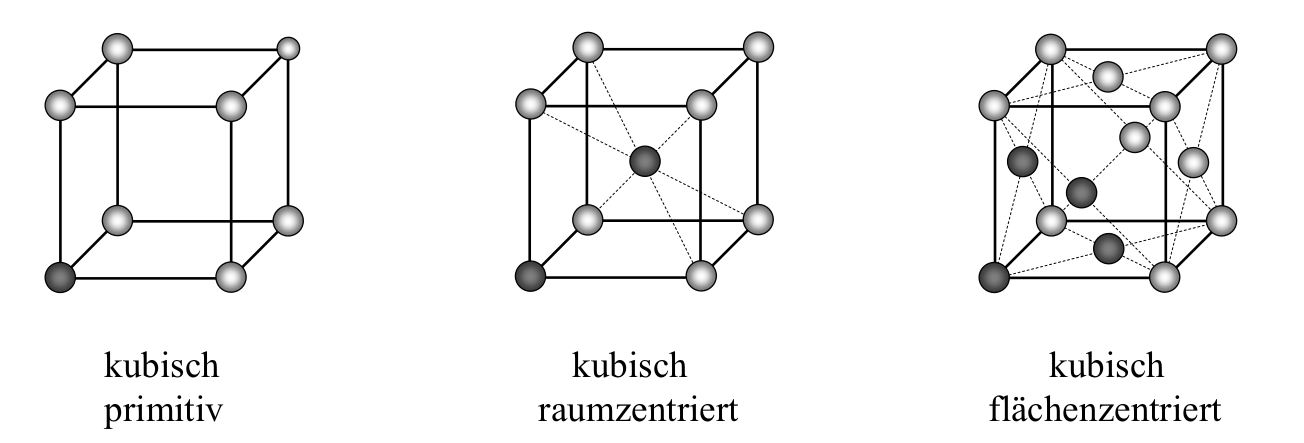
\includegraphics[width=0.9\textwidth]{Abb/kubische_gitter.png}
    \caption{Die drei kubischen Atomgitter. Von links nach rechts: 
             einfach kubisch (sc), kubisch raumzentriert (bcc),
             kubisch flächenzentriert (fcc) \cite{hunklinger}}
    \label{kub}
\end{figure}
Es existieren drei verschiedene kubische Gitter.
Diese sind in Abbildung \ref{kub} dargestellt. Im Rahmen dieses Versuches
soll nur das kubisch flächenzentrierte Gitter näher betrachtet werden. Viele Metalle
und Legierungen kristallisieren in diese Anordnung.\\
\begin{figure}
    \centering
    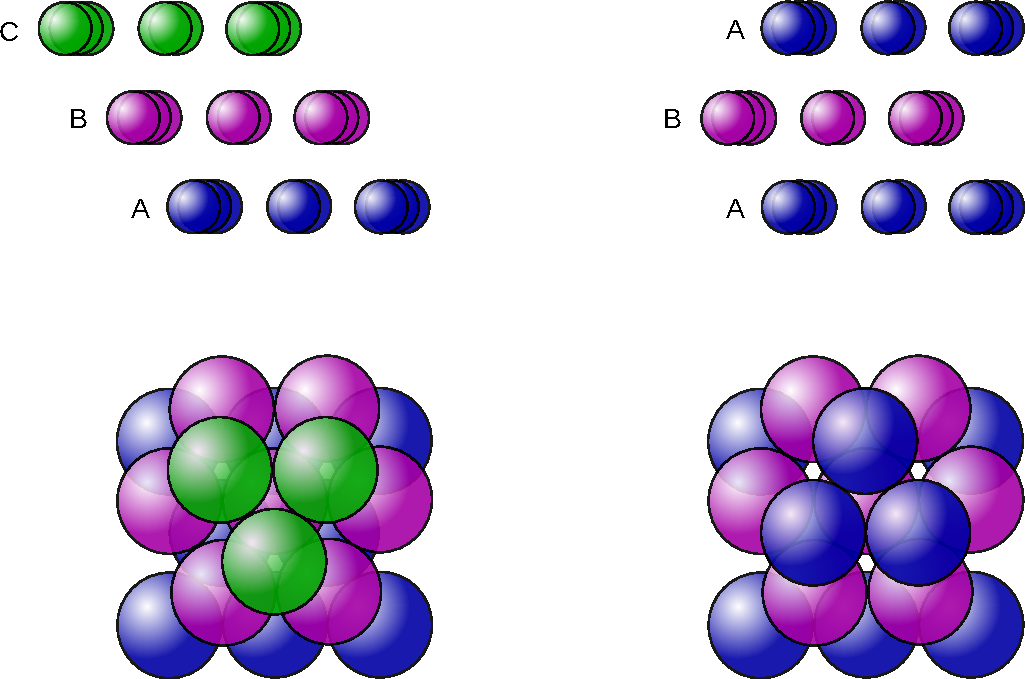
\includegraphics[width=0.7\textwidth]{Abb/DichtesteKugelpackung.pdf}
    \caption{Die möglichen Stapelfolgen für eine dichteste Kugelpackung:
             Links im Bild werden drei verschiedene Schichten gestapelt,
             also ABCABC... 
             Rechts werden nur zwei Schichten gestapelt, die dritte Schicht liegt
             also exakt auf der Ersten, ABABAB... \cite{kugel}}
    \label{pack}
\end{figure}
Betrachtet man eine möglichst dichte Packung an Kugeln, so sind zwei Stapelfolgen 
möglich. Das fcc-Gitter repräsentiert hierbei die Schichtfolge ABCABC..., siehe 
hierzu Abbildung \ref{pack}. Ein Atom hat in dieser Anordnung 12 nächste Nachbarn
mit dem Abstand $\frac{a}{\sqrt{2}}$. $a$ sei hier die Gitterkonstante des Würfels.
In einer kubischer Zelle befinden sich $8 \cdot \frac{1}{8} + 6 \cdot \frac{1}{2} 
= 4$ Atome. Die Atome an den Ecken befinden sich in acht Zellen gleichzeitig, jene 
an den Flächen in zwei. Sie werden deshalb anteilig hinzugerechnet.
Die Packungsdichte $ V_{\text{Atome}} / V_{\text{kub. Zelle}} $ ergibt sich somit zu:
\[
    \underset{\text{Volumen eines Atoms}}{
        \underbrace{
            \frac{4}{3} \left( \frac{d_{NN}}{2} \right)^2 \pi}} \cdot
    \underset{\text{Atome pro kubischer Zelle}}{4} 
    / \, 
    \underset{\text{Volumen des Würfels}}{a^3} \approx 0.74
\]
Die dichtest mögliche Kugelpackung nimmt also $74\%$ des Raums ein.
\newpage

        \subsubsection{Hexagonal dichteste Kugelpackung}

\begin{wrapfigure}{r}{0.45\textwidth}
    \centering
    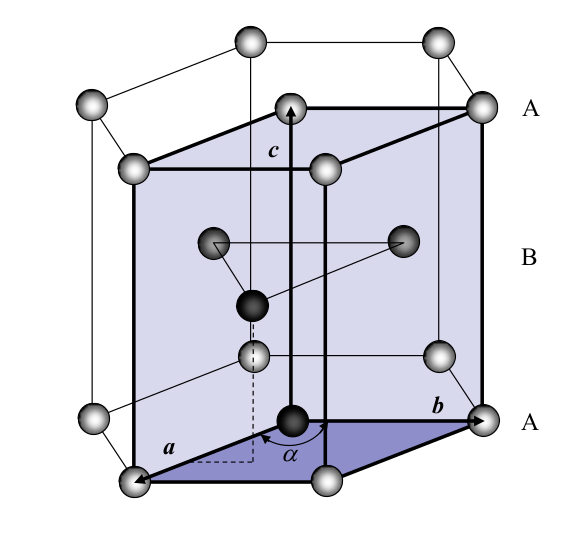
\includegraphics[width=0.4\textwidth]{Abb/hcp.png}
    \caption{hcp-Gitter \cite{hunklinger}}
    \label{hcp}
\end{wrapfigure}
Die rechte Stapelfolge in Abbildung \ref{pack} wird als hexagonal dichteste
Kugelpackung (hcp) bezeichnet. In Eigenschaften wie Abstand und Anzahl der nächsten
Nachbarn gleicht es dem fcc, was durch die Betrachtung als dichteste Packungen 
schnell klar wird. In Abbildung \ref{hcp} sind die Stapelfolgen eingezeichnet.
Die Vektoren $a$ und $b$ sind gleich lang. Für $c$ findet man $c = \sqrt{ 
\frac{8}{3}} \, a$. In realen Kristallen weicht dies oft etwas ab.

     \subsection{Quantenmechanischer Tunneleffekt}

Das Tunneln beschreibt ein quantenmechanischen Effekt, nach dem es für Teilchen
möglich ist eine Energiebarriere zu überwinden, auch wenn diese eine wesentlich
höhere Energie als das Teilchen besitzt. Klassisch wäre dies unmöglich.

        \subsubsection{Theorie des eindimensionalen Tunneleffekts}

Wir betrachten eine Potentialbarriere 
\[
    V(x) = V_0 \Theta ( a - |x| )    
\]
und ein Teilchen mit der Energie $E < V_0$.
\begin{figure}[h]
   \centering
   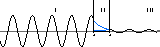
\includegraphics[width=0.9\textwidth]{Abb/tunnel.pdf}
   \caption{Skizze des Tunneleffekts: Die Wellenfunktion des Teilchens läuft von 
            links auf die Potentialbarriere zu. Nach einem exponentiellen Abfall
            im Inneren der Barriere besteht eine kleine Wahrscheinlichkeit, dass
            sich das Teilchen rechts der Barriere aufhält}
   \label{tunnel} 
\end{figure}
Benutzt man die stationäre Schrödingergleichung
\[
    - \frac{\hbar^2}{2m} \frac{d^2}{dx^2} \Phi(x) + V(x) \Phi(x) + V(x) \Phi(x)
    = E \Phi(x)    
\]
so findet sich für die Teilchenwellenfunktion
\[
    \Psi(x) = 
        \begin{cases}
            A \, e^{ikx} + B \, e^{-ikx}, \quad x<-a\\
            C \, e^{-\kappa x} + D \, e^{\kappa x} \quad -a < x < a\\
            F \, e^{ikx} + G \, e^{-ikx}, \quad x<-a
        \end{cases}
\]
mit den Wellenzahlen $k=\sqrt{2mE}/\hbar$ und $\kappa = \sqrt{2m(V_0-E)}/\hbar$.
Benutzt man nun die Anschlussbedingungen
\begin{align*}
    &x=-a: \quad A \, e^{-ika} + B \, e^{ika} = C \, e^{\kappa a} 
        + D \, e^{-\kappa a}\\
    &x=a: \quad F \, e^{+ika} + G \, e^{-ika} = C \, e^{-\kappa a} 
        + D \, e^{+\kappa a}
\end{align*}
und die Normalisierungsbedingung
\[
    \int \Psi^* (x) \Phi (x) dx = 1
\]
so kann man Ausdrücke für die einzelnen Koeffizienten erhalten. Für ein von links 
einfallendes Teilchen, also $G=0$, errechnet sich die Transmissionsamplitude 
$S(E)$ zu
\[
    S(E) = \frac{F}{A} = \frac{e^{-2ika}}{\cosh(2\kappa a) + \frac{i \varepsilon}{2}
                               \sinh(2\kappa a)}
\]
Die Wahrscheinlichkeit einer Transmission, der Durchlässigkeitskoeffizient, 
errechnet sich dann zu
\[
    | S(E) |^2 = \frac{1}{1+(1+(\varepsilon^2/4)) \, \sinh^2(2\kappa a)}
\]
Nimmt man nun eine sehr hohe und breite Barriere an, also $\kappa a >> 1$ und 
vernachlässigt die aus dieser Näherung resultierenden Logarithmusterme, so erhält
man den handlichen Ausdruck
\[
    | S(E) |^2 = \exp\left(-4 \sqrt{2m(V_0-E)} \, \frac{a}{\hbar}\right)
\]

        \subsubsection{Anwendung im Rastertunnelmikroskop}

Zur Abtastung kommt eine scharfe Metallspitze zum Einsatz, die im Abstand weniger
Angstrøm über eine leitfähige Probe positioniert wird. Durch eine angelegte 
Tunnelspannung $U_t$ werden die Fermi-Niveaus der Spitze $E_{F,S}$ und der Probe
$E_{F,P}$ gegeneinander verschoben, schematisch in Abbildung \ref{tunnelstm} 
dargestellt.
\begin{figure}
    \centering
    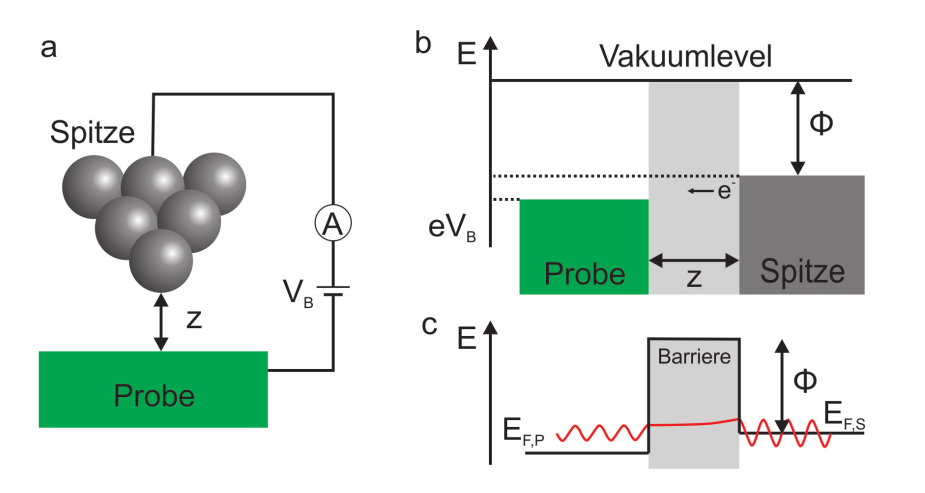
\includegraphics[width=0.8\textwidth]{Abb/tunnel_stm.png}
    \caption{a) Spitze und Probe werden über eine Spannungsquelle und einen 
                Strom-Spannungswandler miteinander verbunden. $V_B$ bezeichnet
                hier die Tunnelspannung, z den Abstand Spitze-Probe.
             b) Die angelegte Spannung verschiebt die beiden Fermi-Niveaus. Bei 
                positiver Spannung tunneln Elektronen der Spitze zur Probe.
             c) Tunneleffekt im STM.
             \cite{hofmann}}
    \label{tunnelstm}
\end{figure}
Der Strom $I_t$ zwischen Spitze und Probe ist nun von $U_t$ und dem Abstand $z$ 
abhängig. Das Abstandverhalten kann nun durch den eindimensionalen Tunnelprozess
hergeleitet werden. Die Höhe der Barriere ist die gemittelte Austrittsarbeit $\Phi$
des Spitzen- und Probenmaterials, also die nötige Energie Elektronen vom jeweiligen
Fermi-Niveau auf Vakuumenergie zu heben. Die Breite der Barriere ist der Abstand $z$.
Typischerweiße ist die angelegte Spannung sehr viel kleiner als $\Phi$, es kann also
eine rechteckige Barriere angenommen werden. Man erhält also:
\[
    I_t = I_0 \cdot e^{-2\kappa z}    
\]
$I_0$ gibt hierbei den Strom bei $z=0$ an und $\kappa = \sqrt{2m \Phi}/ \hbar$, mit
der Elektronenmasse $m$. Für eine typische Austrittsarbeit $\Phi \approx \SI{5}{\eV}$
errechnet sich $I_t \approx \SI{1}{\per \angstrom}$.\\
Für Metalle gilt näherungsweiße:
\[
    I_t \propto U_t \exp(-c_2 \sqrt{\Phi} z)
\]
mit $c_2 = \SI{1,025}{\per\angstrom\per\eV}$.
\cite{schwabl,hofmann}

    \subsection{Piezoelektrischer Effekt}

\begin{wrapfigure}{r}{0.45\textwidth}
    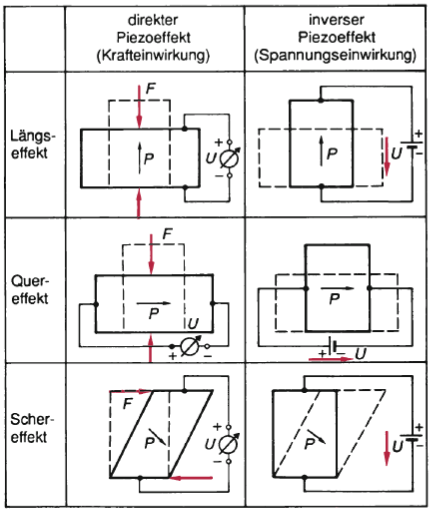
\includegraphics[width=0.45\textwidth]{Abb/piezo.png}
    \caption{Piezoelektrizität \cite{phying}}
    \label{piezo}
\end{wrapfigure}
Bestimmte Materialien erzeugen eine elektrische Spannung, sobald eine äußere Kraft
auf den Körper wirkt. Dies wird als piezoelektrischer Effekt bezeichnet. Er wurde
1880 durch die Brüder Curie an einigen Kristallen entdeckt.\\
Essentiell für die Rastersondenmikroskopie ist der inverse piezoelektrische Effekt.
Dieser führt zu einer Geometrieänderung des Kristalls beim Anlegen einer äußeren 
Spannung. Dies ermöglicht sehr feine Ortsänderungen der Spitze. Es werden drei 
technische nutzbare Vorgänge unterschieden, die in Abbildung \ref{piezo} skizziert
werden.
\begin{itemize}
    \item Längs-Effekt:\\
          Eine äußere Kraft $\textbf{F}$ führt zu einer Polarisierung $\textbf{P}$.
          Die resultierende Spannung $U$ liegt in gleicher Richtung an.
    \item Querr-Effekt:\\
          Eine äußere Kraft $\textbf{F}$ führt zu einer transversalen Polarisation
          $\textbf{P}$. Die resultierende Spannung $U$ liegt nun quer an.
    \item Scher-Effekt:\\
          Eine äußere Kraft $\textbf{F}$ führt zu einer diagonalen Polarisation
          $\textbf{P}$. Die resultierende Spannung $U$ liegt wiederum quer an.
\end{itemize}
Die Anwendungen der Piezoelektrizität sind weitreichend. Abbildung \ref{piezo_anw} 
gibt hierzu eine Übersicht. \cite{phying}
\begin{figure}[H]
    \centering
    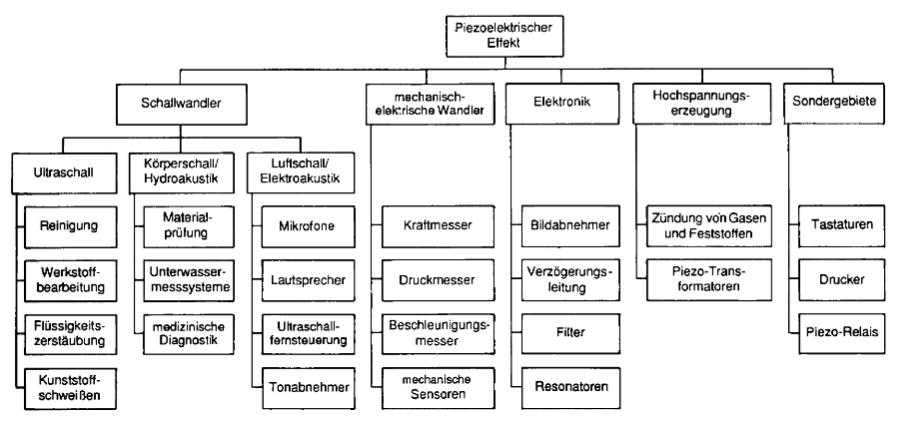
\includegraphics[width=0.9\textwidth]{Abb/piezo_anw.png}
    \caption{Anwendung der Piezoelektrizität \cite{phying}}
    \label{piezo_anw}
\end{figure}

\section{Aufbau eines Rastertunnelmikroskops}
    \subsection{Scanner-Einheit}

\begin{figure}[h]
    \centering
    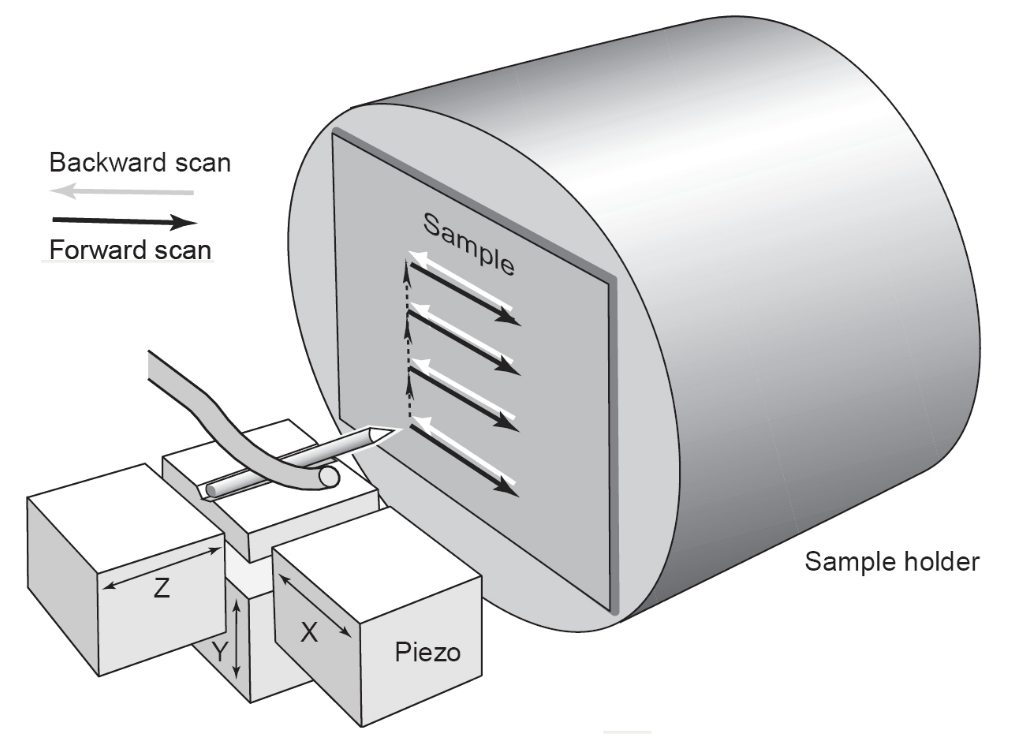
\includegraphics[width=0.7\textwidth]{Abb/scanner.png}
    \caption{Scanner-Einheit eines STM. \cite{nanosurf}}
    \label{scan}
\end{figure}
In Abbildung \ref{scan} ist der schematische Aufbau der Scanner-Einheit gezeigt.
Die leitende Spitze wird durch drei Piezos, pro Raumrichtung ein Piezoelement, 
über der Probe positioniert. Die Längenänderung der Kristalle ist annähernd linear
zur angelegten Spannung. Dies erlaubt eine einfache Steuerung des Aufbaus.

    \subsection{Herstellung der Spitze}

Eine STM-Spitze sollte sehr fein, dünn und starr sein, gleichzeitig auch keine 
Oxidation aufweißen, um möglichst gute Ergebnisse zu erzielen. Zur Herstellung 
wurden demnach zahlreiche Verfahren entwickelt. 

        \subsubsection{Platin-Iridium Spitze}

\begin{figure}[h]
    \centering
    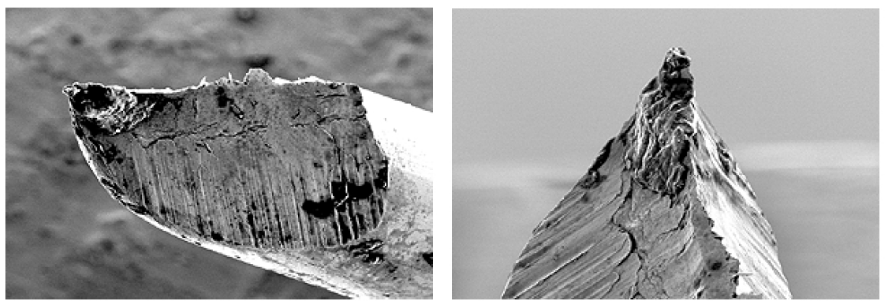
\includegraphics[width=0.7\textwidth]{Abb/pt-ir.png}
    \caption{Pt-Ir Spitze. \cite{nanosurf}}
    \label{ptir}
\end{figure}
Ein sehr einfaches Verfahren bietet die Platin-Iridium Spitze. Zur Herstellung wird
ein dünner Draht mit Zangen ruckartig abgerissen.\\
Die Vorgehensweiße ist in Abbildung \ref{ptirverf} dargestellt. Mit einer Flachzange
wird ein Ende des Drahtes festgehalten. Mit einem Seitenschneider wird unter sehr 
spitzem Winkel angesetzt, bis man Kontakt spürt. Dann wird mit dem Seitenschneider
ruckartig abgerissen.
\begin{figure}[h]
    \centering
    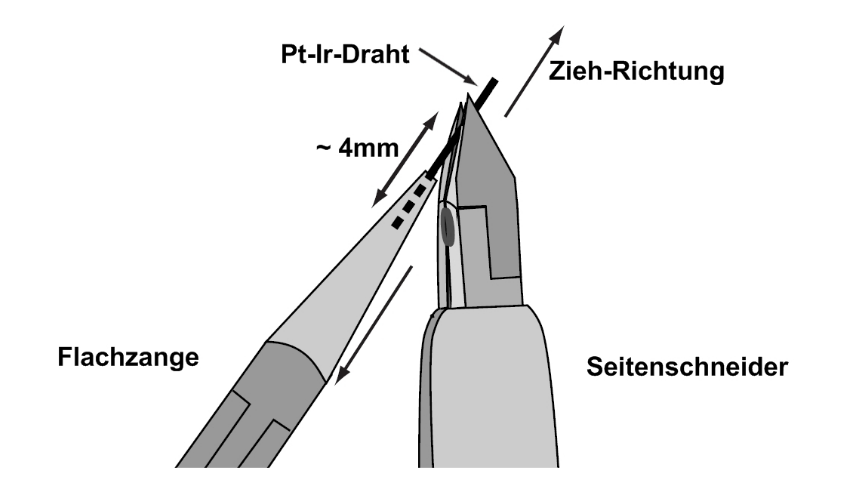
\includegraphics[width=0.6\textwidth]{Abb/pt-it-verf.png}
    \caption{Abreißen eines Platin-Iridiumdrahts. \cite{nanosurf}}
    \label{ptirverf}
\end{figure}
Der große Vorteil dieses Verfahrens ist natürlich die Einfachheit der Herstellung.
Außerdem bietet das Material eine gute Langlebigkeit. Der große Nachteil ist die
Inhomogenität der Beschaffenheit der Spitzen. Durch das zufällige Abreißen 
unterscheidet sich natürlich jede Spitze.

        \subsubsection{Wolfram Spitze}

\begin{figure}[h]
    \centering
    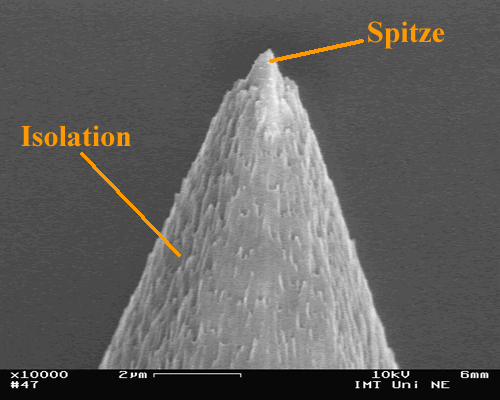
\includegraphics[width=0.6\textwidth]{Abb/wolfram.png}
    \caption{Wolfram Spitze mit Isolation. \cite{wolfram}}
    \label{wolfram}
\end{figure}
Wie in Abbildung \ref{wolfram} zu sehen, sind Wolfram Spitzen wesentlich 
gleichmäßiger als Platin-Iridium Spitzen. Dies ist eine Folge der Herstellung
durch elektrochemisches Ätzen. 
\begin{figure}[h]
    \centering
    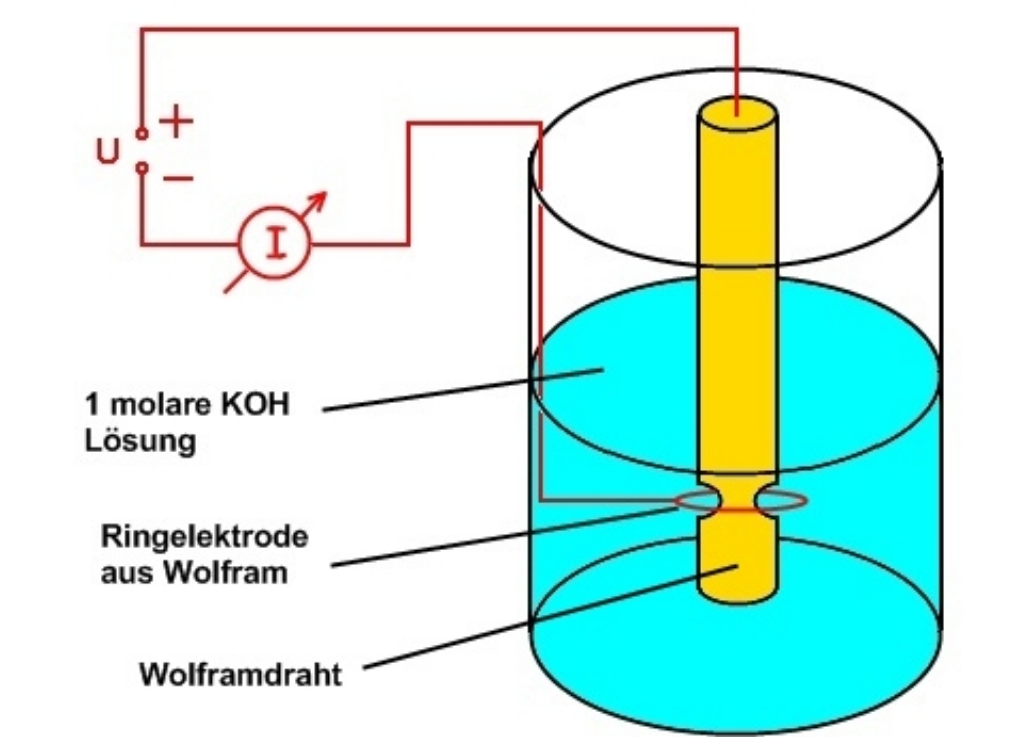
\includegraphics[width=0.6\textwidth]{Abb/wolf_verf.png}
    \caption{Elektrochemisches Ätzen von Spitzen. \cite{beschr}}
    \label{wolf-verf}
\end{figure}
Der Aufbau hierzu ist in Abbildung \ref{wolf-verf} zu sehen. In einer KOH-Lösung 
wandern durch eine angelegte Spannung Wolframatome vom Draht zur Ringelektrode.
Hierbei muss der Wolframdraht positiv und die Ringelektrode negativ gepolt sein,
andernfalls würden sich die Atome an den Draht anlagern. Eine typische Spannung 
ist hier $U \approx \SI{10}{\volt}$. Nach einigen Minuten ist der Wolframdraht
im Bereich der Elektrode durchgeätzt und die beiden resultierenden Teile können 
als Spitze verwendet werden.\\
Der große Vorteil dieses Verfahrens ist die Möglichkeit viele gleichartige Spitzen
herstellen zu können. Allerdings ist die Herstellung aufwendig. Weiter oxidiert 
Wolfram an der Luft schnell, was eine längere Lagerung unterbindet.
\cite{beschr}

\section{Betriebsarten eines Rastertunnelmikroskops}
    \subsection{Topographischer Modus}

\begin{figure}[H]
    \centering
    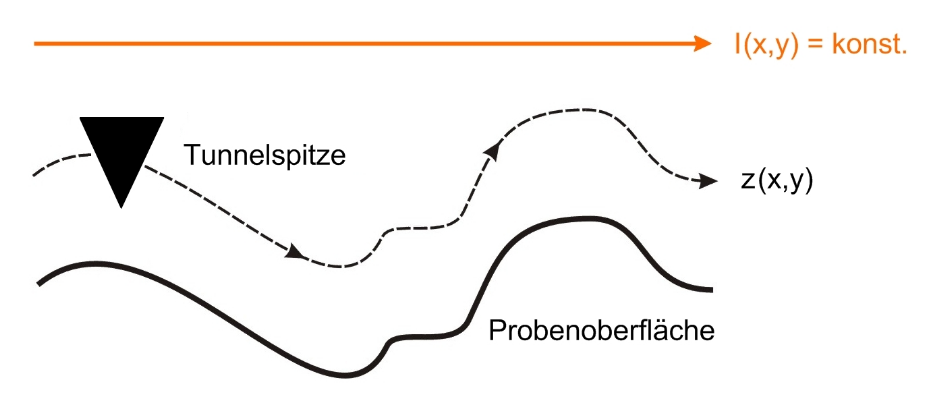
\includegraphics[width=0.8\textwidth]{Abb/topo.png}
    \caption{Topographischer Modus des STM. \cite{beschr}}
    \label{topo}
\end{figure}
Im topographischen Modus folgt die Spitze der Oberflächenbeschaffenheit der Probe,
wie in Abbildung \ref{topo} skizziert. Der Tunnelstrom soll durch Veränderung der 
z-Position beim Abrastern konstant gehalten werden. Das eigentliche Messsignal 
ist dann die Regelspannung des Piezoelements in z-Richtung. Der Nachteil dieser 
Messmethode ist die langsame Scangeschwindigkeit, die aus der ständigen 
Nachjustierung der z-Position resultiert.

    \subsection{Modus konstanter Höhe}

\begin{figure}[h]
    \centering
    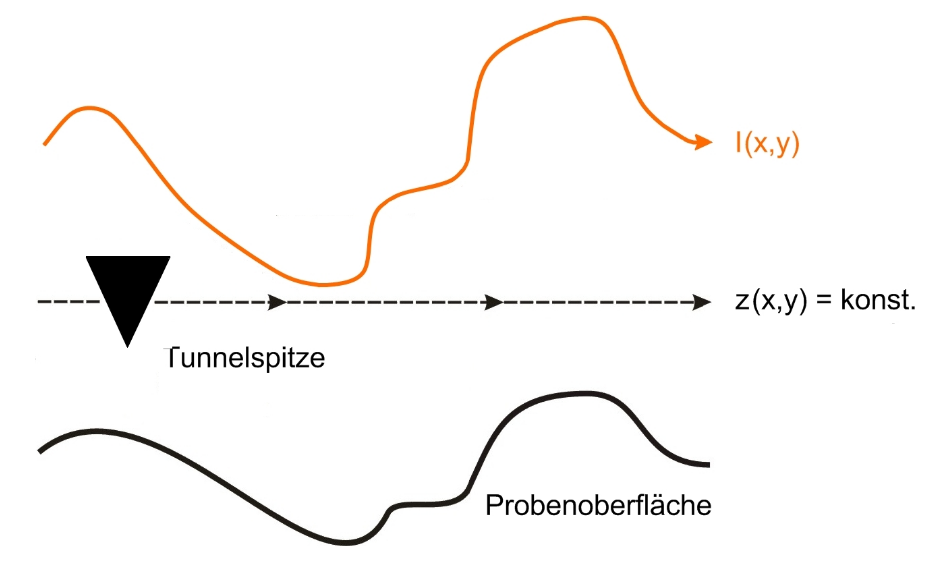
\includegraphics[width=0.7\textwidth]{Abb/konst.png}
    \caption{Modus konstanter Höhe des STM \cite{beschr}}
    \label{konst}
\end{figure}
In diesem Modus rastert die Spitze mit gleichbleibender z-Position, wie in Abbildung
\ref{konst} skizziert. So wird der
sich ändernde Tunnelstrom gemessen und daraus die Oberflächenbeschaffenheit der 
Probe rekonstruiert. Vorteil hierbei ist die hohe Scangeschwindigkeit. Nachteil
ist die Kollissionsgefahr, wodurch Spitze und Probe zerstört werden können. Dieser
Modus wird also nur bei vorheriger Kenntnis der Oberflächenstruktur eingesetzt, um 
nochmals genauere Messungen durchzuführen. Im Rahmen dieses Versuch wird 
ausschließlich der topographische Modus verwendet.

    \subsection{Spektroskopie}

Die Spektroskopie ermöglicht die Messung der lokalen Zustandsdichten (LDOS) der
Probe. Hierzu wird die Position der Spitze relativ zur Probe in allen Raumrichtungen
konstant gehalten. Zusätzlich zur Gleichspannung $U_t$ wird eine Wechselspannung an 
die Spitze angelegt. Unter Variation der Gleichspannung wird nun der Tunnelstrom
gemessen. Zur Auswertung wird der Strom $I_t$ nach der Spannung $U(x,y,U)$ 
aufgetragen. Es gilt:
\[
    I_t \propto \int_0^{eU} \rho_P (E_F - eU + \varepsilon) \; 
                            \rho_S (E_f + \varepsilon) \, d \varepsilon
\]
Dabei gibt $\rho_P$ die Zustandsdichte der Probe und $\rho_S$ die der Spitze an.
Zur Messung von $\rho_P$ muss $\rho_S$ also bekannt sein. Mit $\rho_S$ konstant
ergibt sich:
\[
    \frac{dI}{dU} \propto \rho_P (E_F - eU - \varepsilon)
\]
Die Ableitung der Tunnelstroms nach der Spannung ist also proportional zur 
Zustandsdichten der Probe. 
\cite{beschr}

\section{Probenmaterialien}
    \subsection{Graphit}
    \subsection{Gold}
    \subsection{Molybdänsulfit}